\newpage

\section[Алгоритм выравнивания]{\large \centering Алгоритм выравнивания}
\hspace{\parindent} За основу был взят алгоритм Нидлмана-Вунша и произведена его модификация, благодаря которой заполнение очередной ячейки матрицы происходит с учетом трансляции текущего триплета нуклеотидов в аминокислоту. Таким образом, полученное решение строит двухуровневое выравнивание последовательностей $S_1$ и $S_2$ за время $O(len(S_1)\cdot len(S_2))$. Константа, спрятанная в оценке сложности $O$, равна 25, что позволяет продлить алгоритм до задачи множественного выравнивания.

\subsection[Принятые обозначения]{\large Принятые обозначения}
\hspace{\parindent} Пусть $S_1$ и $S_2$ --- некоторые последовательности нуклеотидов. Введем следующие обозначения:
\begin{itemize}
	\item $len(S_k)$ --- как и в предыдущих пунктах, длина последовательности $S_k$
	\item $S_k[i:j]$ --- подпоследовательность $S_k$ с $i$-го по $j$-ый нуклеотид. Запись $S_k[i:i]$, или просто $S_k[i]$, обозначает $i$-ый нуклеотид $S_k$, а в случае $j < i$ $S_k[i:j]$ является пустой последовательностью
	\item $\mathcal{A}(S_i, S_j)$ --- оптимальное выравнивание последовательностей $S_i$ и $S_j$
	\item $cost(\mathcal{A}(S_i, S_j))$ --- численная характеристика полученного выравнивания, вычисляемая по рекурсивной формуле
	\item $cost('-')$ --- штраф (число) за разрыв последовательности
	\item $cost('!')$ --- штраф за разрыв рамки считывания
	\item $cost('*')$ --- штраф за появление стоп-кодона не в конце последовательности
	\item $\sigma(X, Y)$ --- оценка за сопоставление нуклеотидов (или аминокислот) $X$~и~$Y$
\end{itemize}

\indent Перепишем в новых обозначениях рекурсивную формулу $cost(\mathcal{A}(S_1, S_2))$ для классического алгоритма Нидлмана-Вунша (\ref{eq:N_W_2}).

\begin{equation}\label{eq:N_W_2}
cost(\mathcal{A}(S_1[1:i], S_2[1:j])) = max\left\{
\begin{aligned}
& cost(\mathcal{A}(S_1[1:i-1], S_2[1:j-1]))\\
& \hspace{1cm} + \sigma(S_1[i], S_2[j])\\
& cost(\mathcal{A}(S_1[1:i-1], S_2[1:j]))\\
& \hspace{1cm} + cost('-')\\
& cost(\mathcal{A}(S_1[1:i], S_2[1:j-1]))\\
& \hspace{1cm} + cost('-')
\end{aligned}
\right.
\end{equation}

\indent На каждом шаге рекурсии происходит уменьшение $i$ и/или $j$ на единицу. Условие продолжения рекурсии: $i > 0$ и $j > 0$. Граничные значения при $i=0$ и $j=0$ заполняются по формулам~\ref{eq:N_W_gran}.
\begin{equation}\label{eq:N_W_gran}
\begin{aligned}
cost(\mathcal{A}(-, S_2[1:j])) = j\cdot cost('-')\\
cost(\mathcal{A}(S_1[1:i], -)) = i\cdot cost('-')
\end{aligned}
\end{equation}

\indent Для получения выравнивания необходимо запомнить оптимальный выбор на каждом шаге рекурсии $cost(\mathcal{A}(S_1, S_2))=cost(\mathcal{A}(S_1[1:len(S_1)], S_2[1:len(S_2)]))$ и выполнить восстановление ответа (пункт~\ref{seq:NW}).\\
\indent При построении выравнивания с учетом трансляции нуклеотидов необходимо связать уровни нуклеотидов и аминокислот. Введем дополнительную функцию $\pi(S)$, которая по входной последовательности нуклеотидов $S$ строит ее трансляцию $AA_S$. Трансляция происходит по первой рамке считывания (начиная с первого нуклеотида). Для обозначения неполных кодонов используется символ '!', а стоп-кодоны переводятся в символы '*' без остановки трансляции.\\
\indent Запишем в новых обозначениях рекурсивную формулу $cost(\mathcal{A}(S_1, S_2))$ для алгоритма двухуровневого выравнивания (\ref{eq:AA_2}), рассмотренном в пункте~\ref{NTAAalign}, где $AA_1=\pi(S_1[3i-2:3i])$ и $AA_2=\pi(S_2[3j-2:3j])$.

\begin{equation}\label{eq:AA_2}
cost(\mathcal{A}(S_1[1:3i], S_2[1:3j])) = max\left\{
\begin{aligned}
& cost(\mathcal{A}(S_1[1:3i-3],\\
& \hspace{0.5cm} S_2[1:3j-3])) + \sigma(AA_1, AA_2)\\
& cost(\mathcal{A}(S_1[1:3i-3], S_2[1:j]))\\
& \hspace{0.5cm} + cost('-')\\
& cost(\mathcal{A}(S_1[1:i], S_2[1:3j-3]))\\
& \hspace{0.5cm}  + cost('-')
\end{aligned}
\right.
\end{equation}

В рассмотренных выше алгоритмах используется линейный штраф за разрыв последовательности. Для использования аффинного штрафа введем еще два параметра:
\begin{itemize}
	\item $cost(gap\_open)$ --- штраф за открытие разрыва
	\item $cost(gap\_extension)$ --- штраф за продолжение разрыва
\end{itemize}

\indent Таким образом, за разрыв длины $l$ будет начислен штраф $l\cdot cost('-')$ при линейном или $cost(gap_open) + l\cdot cost(gap_extension)$ --- при аффинном подходе.

\subsection[Построение парного выравнивания]{\large Построение парного выравнивания} \label{PairwiseAlign}
\hspace{\parindent} В отличие от алгоритма Нидлмана-Вунша, учитывающего в своей рекурсивной формуле лишь три варианта перехода (инсерция, делеция или совпадение нуклеотидов), разработанное решение рассматривает дополнительные возможности построения выравнивания с учетом образующихся аминокислот и сдвигов рамки считывания. В некоторых случаях становится выгоднее оставлять друг напротив друга различающиеся нуклеотиды, чтобы в итоге получить одинаковые аминокислоты и не допускать излишних разрывов в последовательности. Кроме этого, сигналом о построении неправильного выравнивания может служить внезапное появление стоп-кодона, на что классические алгоритмы не обращают внимания. На рисунке~\ref{ris:NWvsMULTY} показан пример двух выравниваний, построенных с помощью алгоритма Нидлмана-Вунша и собственного решения. \\
\indent Необходимо отметить, что, регулируя параметры штрафа за открытие и продолжение разрыва в последовательности, а также подобрав определенную матрицу замен нуклеотидов, можно добиться более качественного выравнивания для алгоритма Нидлмана-Вунша на этом тесте, однако, это никак не решает проблем одноуровневого подхода. Для одного набора входных данных выбранные значения будут давать хороший результат, а для другого --- нет. Постоянный подбор оптимальных параметров крайне неэффективен.

\begin{figure}[h]
	\begin{minipage}[h]{0.49\linewidth}
		\center{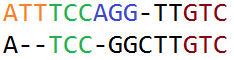
\includegraphics[width=0.9\linewidth]{NW_example} \\ а) Выравнивание по алгоритму Нидлмана-Вунша}
	\end{minipage}
	\hfill
	\begin{minipage}[h]{0.49\linewidth}
		\center{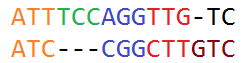
\includegraphics[width=0.9\linewidth]{multy_example} \\ б) Выравнивание по разработанному алгоритму}
	\end{minipage}
	\caption{Пример выравнивания двух последовательностей без учета аминокислотного уровня (а), и с его учетом (б). Одинаковым цветом отмечены одинаковые аминокислоты; неполные кодоны отмечены черным.}
	\label{ris:NWvsMULTY}
\end{figure}

\indent Созданный алгоритм двухуровневого выравнивания на каждом этапе выбора рассматривает все возможные варианты сопоставления от нуля до трех нуклеотидов из каждой последовательности. Таким образом, общее число возможных переходов: $\sum_{i=1}^3 2\cdot 2^i-1=25$. Для наглядности эти варианты представлены на рисунке~\ref{ris:25variants}. 

\begin{figure}[H]
	\begin{minipage}[h]{0.31\linewidth}
		\center{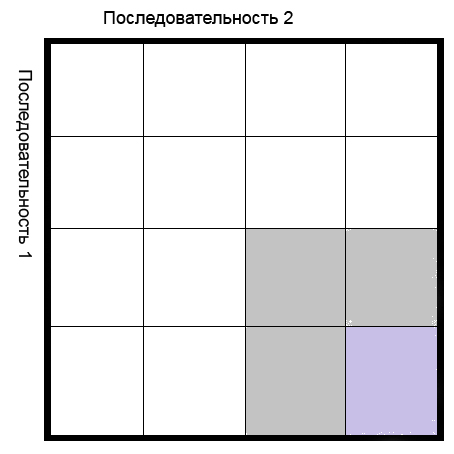
\includegraphics[width=0.95\linewidth]{NT-match} \\ а) Сопоставление нуклеотидов (3~возможных перехода)}
	\end{minipage}
	\hfill
	\begin{minipage}[h]{0.31\linewidth}
		\center{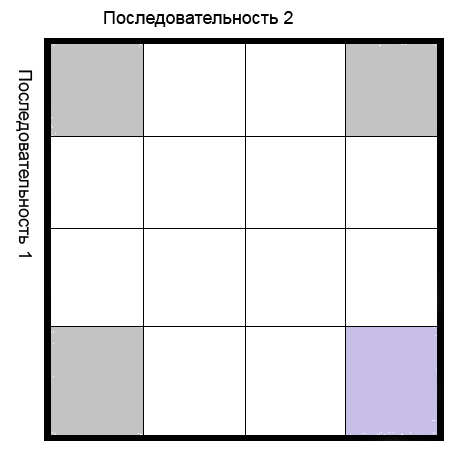
\includegraphics[width=0.95\linewidth]{AA-match} \\ б) Сопоставление аминокислот (3~возможных перехода)}
	\end{minipage}
	\hfill
	\begin{minipage}[h]{0.31\linewidth}
		\center{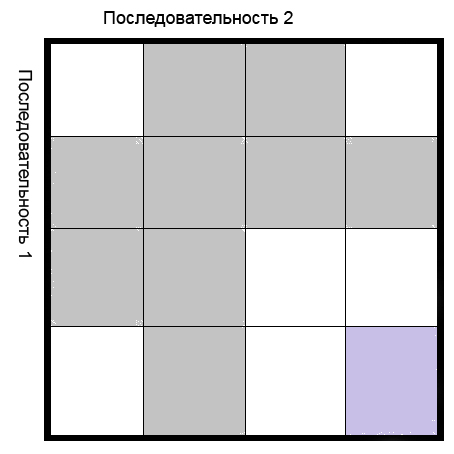
\includegraphics[width=0.95\linewidth]{frame-shift} \\ в) Сопоставление неполных кодонов (19~возможных переходов)}
	\end{minipage}
	\caption{Выбор оптимального шага. Правый нижний угол таблицы представляет собой текущую позицию. Серым выделены рассматриваемые клетки для перехода.}
	\label{ris:25variants}
\end{figure}

\indent При сопоставлении неполных кодонов выходит так много вариантов, потому что до рассматриваемых клеток перехода существует несколько возможных путей. Алгоритм учитывает их все, чтобы гарантировать оптимальное выравнивание на выходе. Ниже представлен псевдокод функции расчета $cost($ $\mathcal{A}(S_1, S_2))$ (листинг~\ref{lst:pairwise}).

\begin{algorithm}[H]
	\caption{Рекурсивный алгоритм построения оптимального парного выравнивания двух кодирующих последовательностей нуклеотидов} \label{lst:pairwise}
	\begin{algorithmic}
		\Procedure{$CalcAlign$}{$S_1, S_2, i, j$}
		\If{i = 0 AND j = 0} \Comment{Проверка граничных условий}
			\State \textbf{return} $0$ 
		\EndIf
		\If{i = 0 OR j = 0} 
			\State \textbf{return} $(i+j-1)*cost(gap\_extension) + cost(gap\_open)$ 
		\EndIf
		\State $AA_1 \gets \pi(S_1[i-2:i])$ \Comment{Трансляция триплетов}
		\State $AA_2 \gets \pi(S_2[j-2:j])$
		\State $stopS_1 \gets 0$
		\State $stopS_2 \gets 0$ \Comment{Проверка на появление преждевременных стоп-кодонов}
		\If{$i \neq len(S_1)$ AND $AA_1 = *$} 
			\State $stopS_1 \gets cost('*')$ 
		\EndIf
		\If{$j \neq len(S_2)$ AND $AA_2 = *$} 
			\State $stopS_2 \gets cost('*')$ 
		\EndIf \Comment{Перебор вариантов: сопоставление аминокислот}
		\State $score \gets max\left\{
		\begin{aligned}
			& CalcAlign(S_1, S_2, i-3, j-3) + \sigma(AA_1, AA_2)\\
			& CalcAlign(S_1, S_2, i-3, j) + stopS_1 + cost('-')\\
			& CalcAlign(S_1, S_2, i, j-3) + stopS_2 + cost('-')\\
		\end{aligned}
		\right.$ 
		\Statex \Comment{Перебор вариантов: сопоставление неполных триплетов}
		\State $score \gets max\left\{
		\begin{aligned}
			& CalcAlign(S_1, S_2, i-2, j-2) + \sigma(S_1[i-1], S_2[j-1]) \\ 
			& \hspace{1cm}+ \sigma(S_1[i], S_2[j]) + 2\cdot cost('!')\\
			& CalcAlign(S_1, S_2, i-2, j-1)\\
			& \hspace{1cm}+ \sigma(S_1[i-1], S_2[j]) + 2\cdot cost('!')\\
			& CalcAlign(S_1, S_2, i-2, j-1)\\
			& \hspace{1cm}+ \sigma(S_1[i], S_2[j]) + 2\cdot cost('!')\\
			& CalcAlign(S_1, S_2, i-2, j) + cost('!') + cost('-')\\
			& CalcAlign(S_1, S_2, i-1, j-2)\\
			& \hspace{1cm}+ \sigma(S_1[i], S_2[j-1]) + 2\cdot cost('!')\\
			& CalcAlign(S_1, S_2, i-1, j-2)\\
			& \hspace{1cm}+ \sigma(S_1[i], S_2[j]) + 2\cdot cost('!')\\
			& score
		\end{aligned}
		\right.$
		\algstore{bkbreak}
	\end{algorithmic}
\end{algorithm}

\begin{algorithm}
	\begin{algorithmic}
		\algrestore{bkbreak}
		\State $score \gets max\left\{
		\begin{aligned}	
			& CalcAlign(S_1, S_2, i, j-2) + cost('!') + cost('-')\\
			& CalcAlign(S_1, S_2, i-3, j-2) + \sigma(S_1[i-2], S_2[j-1])\\ 
			& \hspace{1cm} + \sigma(S_1[i-1], S_2[j]) + stopS_1 + cost('!')\\
			& CalcAlign(S_1, S_2, i-3, j-2) + \sigma(S_1[i-1], S_2[j-1])\\ 
			& \hspace{1cm} + \sigma(S_1[i], S_2[j]) + stopS_1 + cost('!')\\
			& CalcAlign(S_1, S_2, i-3, j-2) + \sigma(S_1[i-2], S_2[j-1])\\ 
			& \hspace{1cm} + \sigma(S_1[i], S_2[j]) + stopS_1 + cost('!')\\
			& CalcAlign(S_1, S_2, i-3, j-1) + \sigma(S_1[i-2], S_2[j])\\
			& \hspace{1cm} + stopS_1 + cost('!')\\
			& CalcAlign(S_1, S_2, i-3, j-1) + \sigma(S_1[i-1], S_2[j])\\
			& \hspace{1cm} + stopS_1 + cost('!')\\
			& CalcAlign(S_1, S_2, i-3, j-1) + \sigma(S_1[i], S_2[j])\\
			& \hspace{1cm} + stopS_1 + cost('!')\\
			& CalcAlign(S_1, S_2, i-2, j-3) + \sigma(S_1[i-1], S_2[j-2])\\ 
			& \hspace{1cm} + \sigma(S_1[i], S_2[j-1]) + stopS_2 + cost('!')\\
			& CalcAlign(S_1, S_2, i-2, j-3) + \sigma(S_1[i-1], S_2[j-1])\\ 
			& \hspace{1cm} + \sigma(S_1[i], S_2[j]) + stopS_2 + cost('!')\\
			& CalcAlign(S_1, S_2, i-2, j-3) + \sigma(S_1[i-1], S_2[j-2])\\ 
			& \hspace{1cm} + \sigma(S_1[i], S_2[j]) + stopS_2 + cost('!')\\
			& CalcAlign(S_1, S_2, i-1, j-3) + \sigma(S_1[i], S_2[j-2])\\
			& \hspace{1cm} + stopS_2 + cost('!')\\
			& CalcAlign(S_1, S_2, i-1, j-3) + \sigma(S_1[i], S_2[j-1])\\
			& \hspace{1cm} + stopS_2 + cost('!')\\
			& CalcAlign(S_1, S_2, i-1, j-3) + \sigma(S_1[i], S_2[j])\\
			& \hspace{1cm} + stopS_2 + cost('!')\\
			& score
		\end{aligned}
		\right.$
		\Statex \Comment{Перебор вариантов: сопоставление нуклеотидов}
		\State $score \gets max\left\{
		\begin{aligned}
			& CalcAlign(S_1, S_2, i-1, j-1) + \sigma(S_1[i], S_2[j])\\
			& \hspace{1cm} + 2\cdot cost('!')\\
			& CalcAlign(S_1, S_2, i-1, j) + cost('!') + cost('-')\\
			& CalcAlign(S_1, S_2, i, j-1) + cost('!') + cost('-')\\
			& score\\
		\end{aligned}
		\right.$
		\State \textbf{return} $score$
		\EndProcedure
	\end{algorithmic}
\end{algorithm}

\indent Необходимо отметить, что при построении ответа нужно делать восстановление рамки в тех случаях, когда алгоритм выбрал в качестве оптимального шага сопоставление неполных триплетов (рисунок~\ref{ris:NotCompleteCodons}).

\begin{figure}[h]
	\center{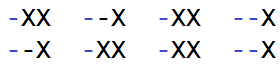
\includegraphics[width=0.6\linewidth]{not-complete-codons.png}}
	\caption{Сопоставление неполных триплетов. Цветом указаны разрывы, добавленные для сохранения текущей рамки считывания.}
	\label{ris:NotCompleteCodons}
\end{figure}

\subsection[Алгоритм кластеризации]{\large Алгоритм кластеризации}
\hspace{\parindent} Для построения множественного выравнивания используется идея выравнивания выравниваний (пункт~\ref{align-align}). Порядок объединения последовательностей определяется по методу невзвешенного попарного среднего (UPGMA --- Unweighted Pair Group Method with Arithmetic mean) \cite{legendre1998numerical}. Для использования этого алгоритма кластеризации необходимо определить функцию расстояния между выравниваемыми строками: $dist(S_i, S_j) \rightarrow \mathbb{R}$. Последовательность $S_1$ ближе к последовательности $S_2$, чем к $S_3$, если $dist(S_1, S_2) > dist(S_1, S_3)$. Чем выше значение $dist(S_i, S_j)$, тем более похожими считаются строки $S_i$~и~$S_j$.\\
\indent В качестве функции расстояния можно использовать $cost(\mathcal{A}(S_i, S_j))$, однако, ее вычисление требует больших вычислительных ресурсов. Альтернативный подход к оценке похожести двух строк --- сравнение их подстрок фиксированной длины.\\
\indent Пусть имеются две последовательности $S_1$ и $S_2$. Рассмотрим все их подстроки длины~$k$: $S_1[i: i+k-1] \in A_1, i = 1\dots len(S_1)-k+1$ и $S_2[i: i+k-1] \in A_2, i = 1\dots len(S_2)-k+1$. Расстояние между последовательностями --- это количество одинаковых подпоследовательностей $dist(S_1, S_2) = |A_1\cap A_2|$. Данный метод имеет меньшую точность, по сравнению с построением оптимального парного выравнивания, однако, он проще и требует меньше операций вычисления при небольших значениях $k$.\\
\indent На начальном этапе алгоритма кластеризации происходит вычисление расстояния между всеми последовательностями, заполняется таблица $D=dist(S_i, S_j)$ $i,j=1 \dots n$. Далее, на каждом шаге из матрицы $D$ выбирается максимальное значение, которое определяет текущие кластеры $i$ и $j$ для объединения, после чего происходит пересчет расстояний от нового кластера до всех остальных по формуле~\ref{eq:upgma} 

\begin{equation}\label{eq:upgma}
D((i,j), w)=\frac{T_iD(i,w)+T_jD(j,w)}{T_i+T_j}
\end{equation}
где $T_k$ --- количество последовательностей в кластере $k$. Старые $i$ и $j$ столбцы и строки таблицы $D$ становятся недействительными. Таким образом, с каждой новой итерацией алгоритма происходит уменьшение числа кластеров на единицу: два кластера собираются в один. Финальное объединение двух последних кластеров даст итоговое выравнивание, содержащее все исходные последовательности нуклеотидов. На рисунке~\ref{ris:UPGMA} представлен пример работы алгоритма.
\begin{figure}[h]
	\center{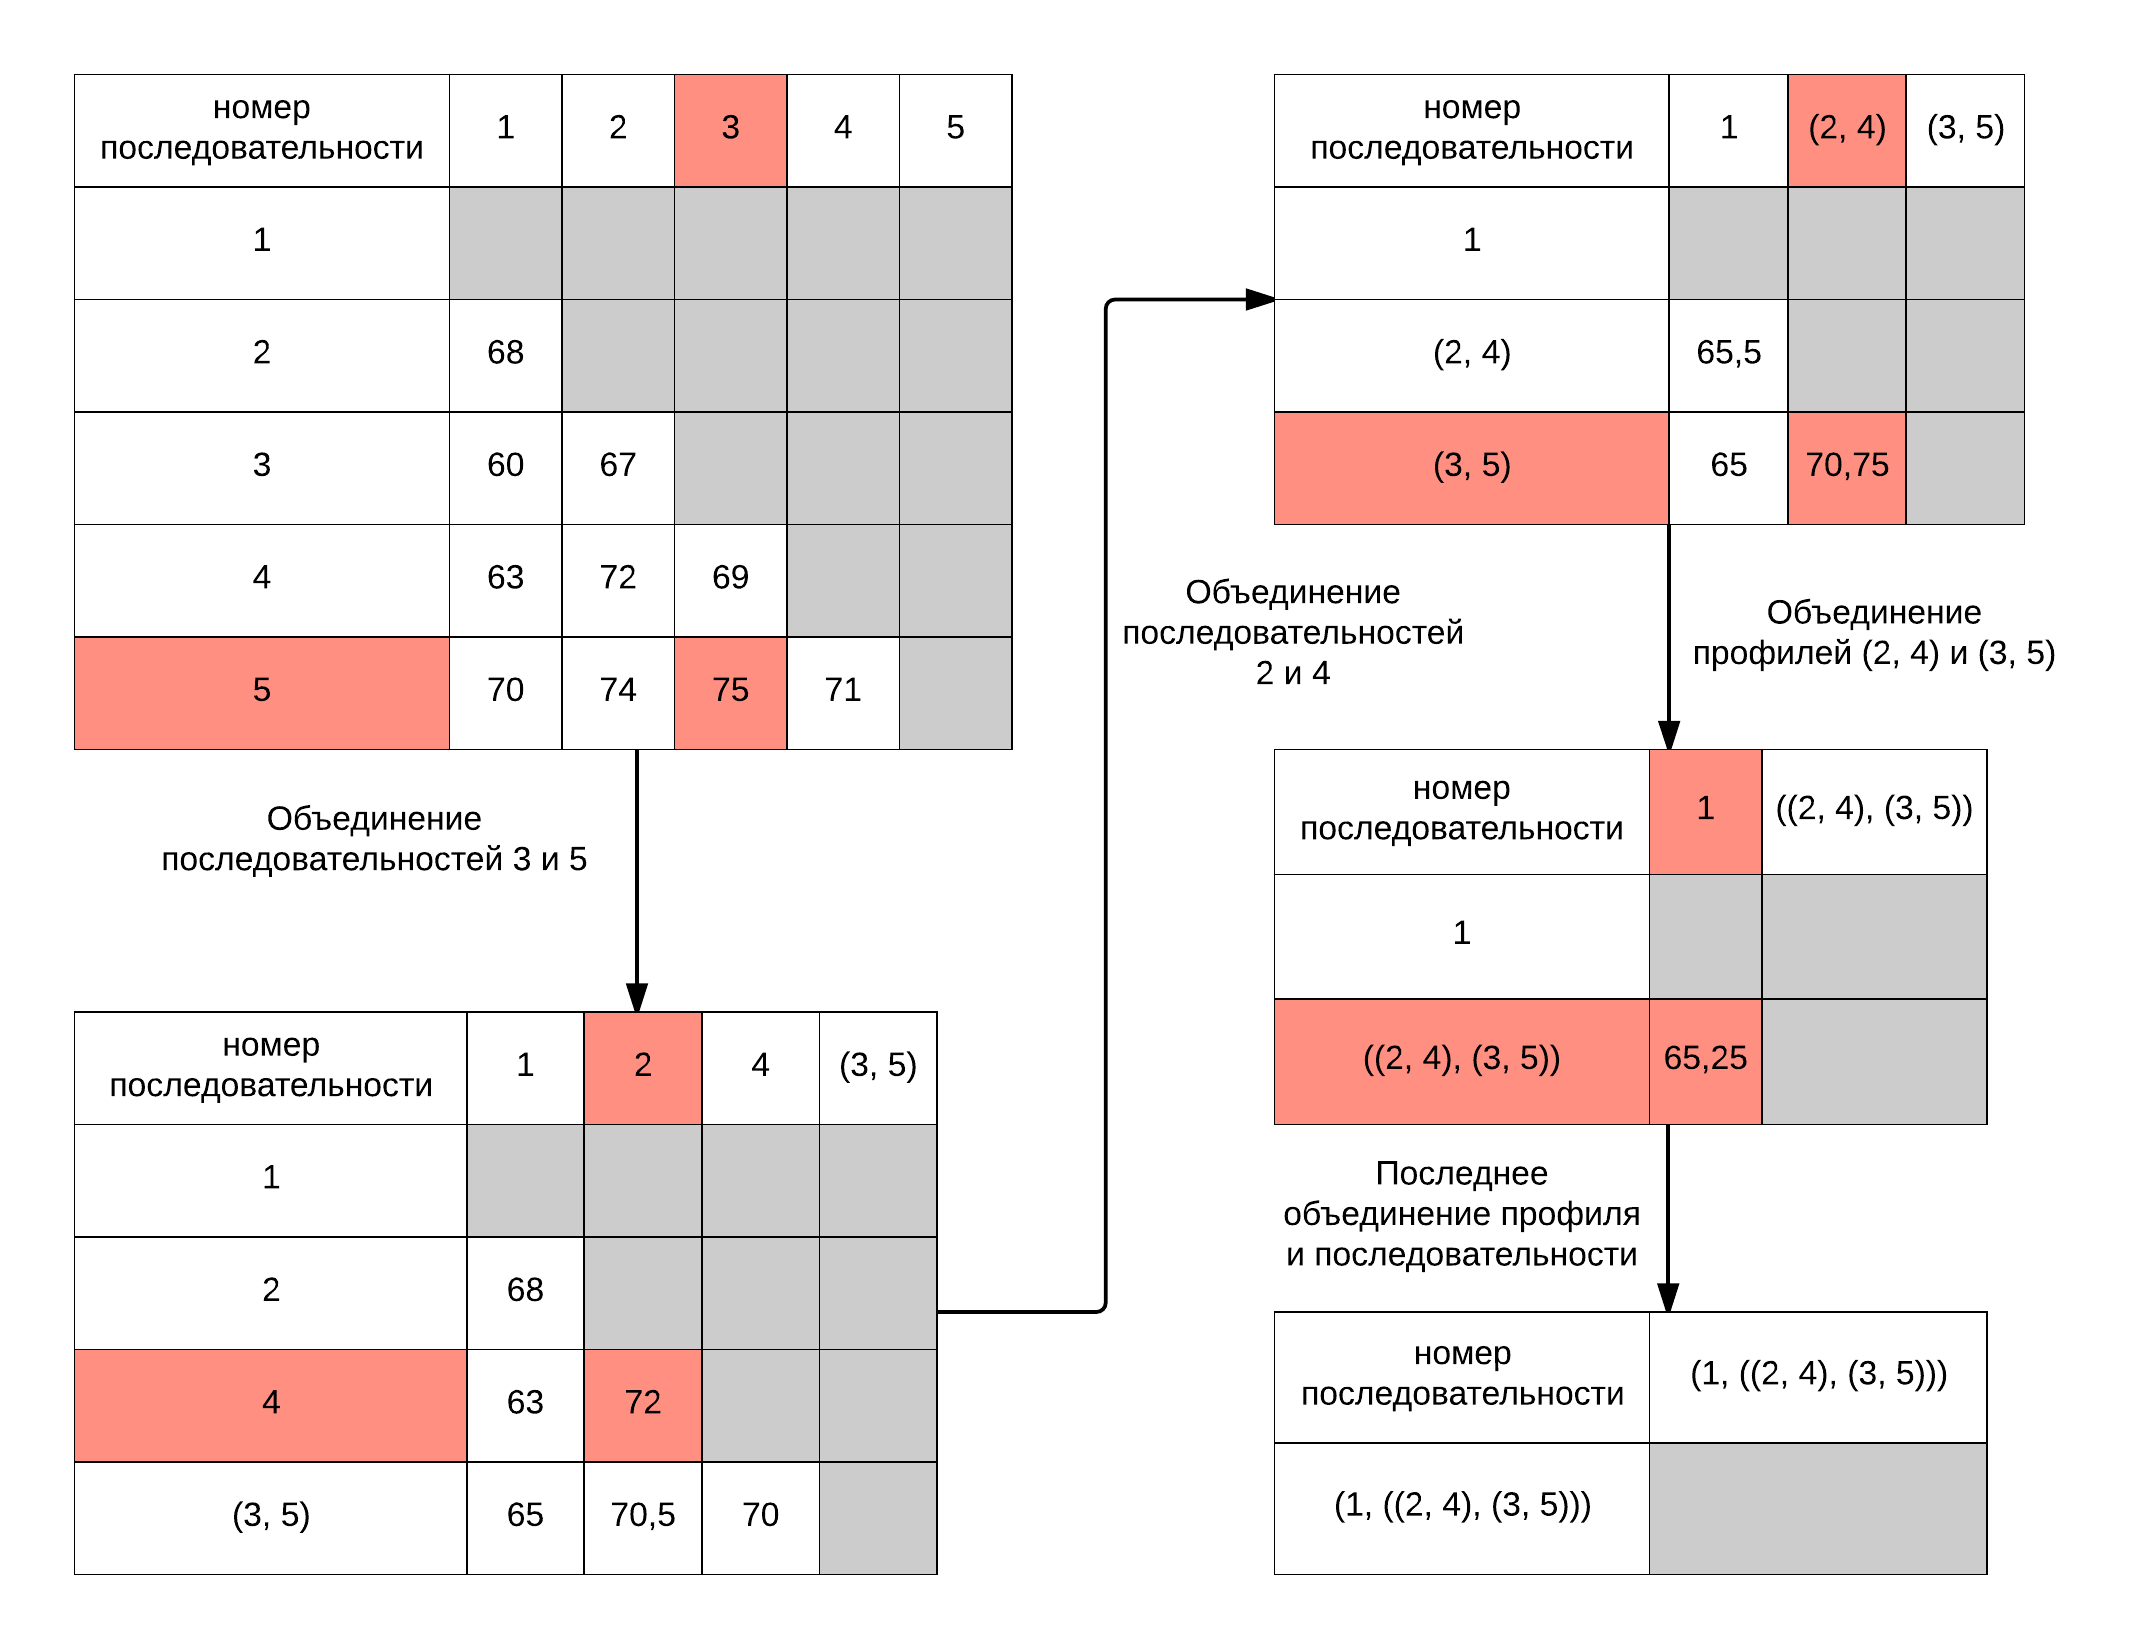
\includegraphics[width=0.95\linewidth]{UPGMA.png}}
	\caption{Изменение матрицы расстояний в процессе кластеризации. Красным цветом обозначены объединяемые кластеры.}
	\label{ris:UPGMA}
\end{figure}

\indent Необходимо отметить, что процесс кластеризации необязательно продолжать до объединения всех кластеров в один. Если найденный в таблице $D$ максимум чересчур мал, то это свидетельствует о слабом родстве последовательностей, и, чтобы не испортить построенное выравнивание, алгоритм можно остановить.

\subsection[Построение множественного выравнивания]{\large Построение множественного выравнивания}
\hspace{\parindent} Введем обозначение <<профиль>> $P$ как набор выравненных строк. Используя рассмотренный выше алгоритм парного выравнивания, можно объединять две последовательности в один профиль $P_{12}=\mathcal{A}(S_1, S_2)$. Для построения множественного выравнивания необходимо ввести операции сложения профилей $P_i + P_j$ и профиля со строкой $P_i + S_j$.\\
\indent При переходе от последовательностей к профилям достаточно определиться с интерпретацией $\sigma(P_1[i], P_2[j])$/$\sigma(P_1[i], S_2[j])$ и $\sigma(\pi(P_1[i-2:i]),$ $\pi(P_2[$ $j-2:j]))$/$\sigma(\pi(P_1[i-2:i]), \pi(S_2[j-2:j]))$, чтобы использовать алгоритм парного выравнивания для операций объединения. В отличие от строки, у профиля по $i$-ой позиции находится набор нуклеотидов из всех входящих в него последовательностей по $i$-ому индексу (рисунок~\ref{ris:profile}). Для каждого такого столбца $i=1 \dots len(P)$, где $len(P)$ --- длина профиля, можно рассчитать частоты встречающихся символов.

\begin{figure}[h]
	\center{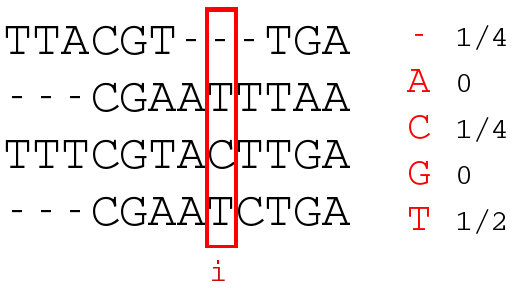
\includegraphics[width=0.8\linewidth]{profile.png}}
	\caption{Профиль из четырех последовательностей и распределение частот для $i$-го столбца}
	\label{ris:profile}
\end{figure}

Тогда определим $\sigma(P[i], S[j])$ по формуле~\ref{eq:freq}, где $\lambda_i[N]$ --- частота нуклеотида $N$ в $i$-ом столбце профиля $P$.

\begin{equation}\label{eq:freq}
\sigma(P[i], S[j])=\sigma('A', S[j])\lambda_i['A']+\sigma('C', S[j])\lambda_i['C']+ \dots +\lambda_i['-']cost('-')
\end{equation}

Аналогичным образом вычисляется $\sigma(\pi(P[i-2:i]), \pi(S[j-2:j]))$, только в данном случае $\lambda_{i-2:i}$ содержит частоты распределения аминокислот в профиле.\\
\indent В случае объединения двух профилей необходимо рассчитать частоты для каждого из них $\lambda_i$ и $\lambda_j$, после чего произвести полный перебор по всем возможным вариантам сопоставления, как в формуле~\ref{eq:freq}. Результат вычислений нормируется, чтобы счет за сопоставление столбцов никак не зависел от количества последовательностей в профилях.\\
\indent Таким образом, итоговый алгоритм множественного выравнивания производит объединение исходных строк в профили, определяя порядок по алгоритму кластеризации. Для сложения профилей и строк используется алгоритм парного двухуровневого выравнивания.